\section{Human Evaluation Studies}
\label{sec:app_human}

Automated metrics measure textual and statistical surface properties; they do not test whether LLAMIA's internalized representations produce game understanding that is perceptually meaningful to a skilled chess player. We conduct two human studies to address this directly: a \emph{gameplay identification study} (Study~1) testing whether LLAMIA's move choices are stylistically distinguishable from human play, and a \emph{commentary quality study} (Study~2) testing whether LLAMIA's commentary conveys more accurate strategic insight than the verbalized baseline and whether it enables readers to form more accurate board evaluations.

% =============================================================================
\subsection{Participants}
\label{sec:app_human_participants}

We recruited $n_0 = 14$ participants from university chess club chapters via in-person announcement at weekly club meetings. Eligibility required either a current FIDE rating or a verified Chess.com or Lichess rapid rating $\geq 1700$ with $\geq 200$ rated games on record.  Following the calibration task described below, $n = 12$ participants met the inclusion criterion and proceeded to both studies.

Both human studies were conducted under a protocol approved by the Institutional Review Board (IRB).
Participants were recruited voluntarily and provided written informed consent prior to enrollment. The consent form described the study purpose, the nature of all tasks,  and the intended use of collected data. Participants were informed that some game segments and commentary samples were AI-generated.

Session data (gameplay judgments, Likert ratings, and open-text responses) were anonymized at the point of collection. Each participant was assigned a randomized identifier; no names, handles, or affiliations were retained in the analysis dataset. Raw recordings were deleted following transcription. Participant data will not be shared in identifiable form.

% =============================================================================
\subsection{Sensitivity Calibration and Participant Selection}
\label{sec:app_human_calibration}

A participant's ability to evaluate AI gameplay depends on their sensitivity to stylistic differences between human and engine play, not only their rating. We screen for this explicitly before the main studies.

\paragraph{Design.}
Each participant reviews 20 recorded game segments in randomized order. Ten segments are drawn from human-vs.-human games (negative controls); the remaining ten from human-vs.-bot games in which the bot is Stockfish~17 at varied strength levels ($n = 3$), Maia ($n = 4$), or a weaker rule-based engine ($n = 3$). For each segment, the participant identifies which player (White or Black) is the bot via forced binary choice; human-vs.-human segments include a ``Neither'' option. Both positive and negative controls are required to measure true discrimination sensitivity rather than a bias to label any player as a bot.

\paragraph{Inclusion criterion.}
Participants achieving $\geq 70\%$ overall accuracy ($\geq 14{/}20$ correct) proceed to the main studies. Of $n_0 = 14$ recruited participants, $n = 12$ met this criterion. The 12 included participants achieved a median calibration accuracy of 75\%.

% =============================================================================
\subsection{Study 1: Gameplay Identification}
\label{sec:app_human_gameplay}

\paragraph{Stimuli.}
We construct 30 game segments from held-out games in the LLAMIA-Bench evaluation set. Each segment comprises 10 consecutive half-moves (5 per side), drawn equally from middlegame and endgame phases (15 segments each). Opening segments are excluded: early-game play is dominated by memorized theory and reveals little about model behaviour. Segment boundaries are defined by board position (middlegame: $\geq 6$ pieces per side, material $\geq 20$ points; endgame: $\leq 5$ pieces per side or rook-and-pawn endings). Two players per segment are labeled Player~A and Player~B; one is drawn from a game involving LLAMIA, LLAMIA-Verb-14B, or a human player. Segments are rendered as fixed-speed board replays (3 seconds per half-move) with clock information removed to prevent trivial detection via time usage.

\paragraph{Task.}
For each segment, participants respond to three prompts:
\begin{enumerate}[leftmargin=*, itemsep=2pt]
  \item \textbf{Bot identification} (primary): ``Which player, A or B, do you believe is the AI?''\ (Forced choice; human-vs.-human segments include ``Neither.'')
  \item \textbf{Confidence} (1--5 scale): ``How confident are you in this judgment?''
  \item \textbf{Open commentary} (free text): ``Which specific moves or patterns informed your decision?''
\end{enumerate}

\paragraph{Design.}
Each participant evaluates 10 segments randomly drawn from the pool of 30, keeping total session time to 40--50 minutes. Assignment is balanced so that every segment receives at least 4 independent judgments. Following bot identification, participants rate their gameplay experience for each segment they played:
\begin{enumerate}[leftmargin=*, itemsep=2pt]
  \item \textbf{Human-likeness} (1--5 Likert): ``My opponent played like a human player.''
  \item \textbf{Enjoyment} (1--5 Likert): ``I enjoyed this game.''
\end{enumerate}
These subjective ratings provide convergent evidence alongside the objective detection accuracy: a system that is both hard to detect and rated as human-like in experience achieves qualitative human-likeness, not merely move-distribution similarity.

\somesh{do we need this?}
\paragraph{Qualitative coding.}
Open-text responses are transcribed and coded along four dimensions by two independent annotators: (i)~\emph{tactical cues}---references to captures, checks, or forcing sequences; (ii)~\emph{positional cues}---references to pawn structure, piece activity, or long-term plans; (iii)~\emph{stylistic cues}---references to move tempo, unnatural patterns, or ``computer-like'' consistency; (iv)~\emph{no identifiable cue}---the participant could not articulate a reason. Inter-annotator agreement is reported as Cohen's $\kappa$. This qualitative layer distinguishes tactical imitation from deeper stylistic assimilation: a system that merely selects strong moves will produce tactical cues; a system whose move distribution lacks non-human regularities will produce no-cue responses.

\paragraph{Primary metric.}
Bot detection accuracy per system: the fraction of segments in which the participant correctly identifies the AI-controlled player. Lower accuracy on LLAMIA segments indicates a move distribution less readily distinguished from human play.

% =============================================================================
\subsection{Study 2: Commentary Quality}
\label{sec:app_human_commentary}

\paragraph{Stimuli.}
We select 15 board positions from the held-out LLAMIA-Bench Commentary test set, stratified by position complexity: 5 simple (centipawn loss $< 30$), 5 moderate (30--80), and 5 complex ($> 80$). Positions are drawn from the same middlegame and endgame phases as Study~1. For each position, commentary is generated from all systems in the LLAMIA-Bench evaluation suite. Commentary operates at the position level---a single move and its strategic rationale---to isolate single-position reasoning and avoid narrative continuity confounds. For the preference and Likert tasks, participants see LLAMIA-14B and LLAMIA-Verb-14B side-by-side, labeled ``System~A'' and ``System~B'' with left-right assignment independently randomized. For the comparative state annotation task, each system's commentary is presented individually. Every participant evaluates all 15 positions, yielding a fully crossed design ($n = 12$ raters $\times$ 15 positions $= 180$ total judgments).

\paragraph{Dimensions.}
Accuracy and Insight are the two scored dimensions. If latent state internalization gives LLAMIA access to richer engine representations than verbalization permits, the difference should manifest as greater factual accuracy (grounded in actual evaluation) and greater strategic depth (conveying non-obvious plans). Fluency and engagement are excluded: both systems produce grammatical prose, and metrics insensitive to chess content are unlikely to discriminate.

\paragraph{Task.}
For each position (estimated 3--4 minutes), participants complete four items:
\begin{enumerate}[leftmargin=*, itemsep=2pt]
  \item \textbf{Overall preference} (forced choice with escape): System~A / System~B / No clear preference.
  \item \textbf{Accuracy} (1--5 Likert): ``The commentary correctly describes what is happening on the board.''
  \item \textbf{Insight} (1--5 Likert): ``The commentary reveals something strategically non-obvious about this position.''
  \item \textbf{Comparative state annotation}: After reading each system's commentary for a middlegame position, the participant predicts the board evaluation on a 7-point scale ($-3$ = Black winning clearly, $0$ = equal, $+3$ = White winning clearly). Administered per-system across all systems. Correctness is Pearson $r$ between predicted and actual Stockfish centipawn evaluations, averaged across raters.
\end{enumerate}

\paragraph{Primary metrics.}
(i)~Preference rate for LLAMIA: fraction of judged pairs (excluding ``no clear preference'') choosing the LLAMIA output, reported as a mean across 12 raters. (ii)~Mean Accuracy and Insight Likert scores per system. (iii)~Pearson $r$ with Stockfish per system.

\paragraph{Rater--judge agreement.}
All 180 position pairs are independently scored with GPT-4o G-eval \citep{liu2023gevalnlgevaluationusing} using matched Accuracy and Insight prompts. Cohen's $\kappa$ is computed between human preference rankings and G-eval rankings, with a length-adjusted $\kappa$ computed after partialling out the Spearman correlation between G-eval score and commentary word count ($\rho_{\text{length}}$).

% =============================================================================
\subsection{Results}
\label{sec:app_human_results}

% ── Study 1 ──────────────────────────────────────────────────────────────────
\paragraph{Study 1 -- Bot detection accuracy.}
Participants correctly identified LLAMIA-14B as the AI-controlled player in only 39\% of trials, below the 50\% chance level---yielding a human-pass rate of 61\%. LLAMIA-Verb-14B was detected in 72\% of trials (human-pass rate 28\%), well above chance. Confidence ratings were lower for LLAMIA-14B segments (mean 2.6 vs.\ 3.4), indicating that near-chance detection reflects genuine perceptual ambiguity rather than participant disengagement. Catch-trial accuracy (human-vs.-human ``Neither'' responses) was 83\%, confirming that participants withheld bot identification when none was warranted.

The detection gap is specific to the integration mode, not the backbone or training recipe. LLAMIA-Verb-14B uses the same Qwen3-14B backbone and the same DAPO training budget; its higher detectability is associated with the verbalization interface: verbal summaries impose regularities on move selection---consistent avoidance of dubious moves, move-tempo patterns---that participants identify as non-human. LLAMIA-14B, reasoning over latent representations, produces a move distribution that does not exhibit these regularities.

Qualitative coding ($\kappa_{\text{code}} = 0.72$) confirms this interpretation. The dominant detection cue for LLAMIA-Verb-14B segments was \emph{stylistic} (65\%: ``moves felt too consistent,'' ``never played a dubious move''). LLAMIA-14B segments produced \emph{no-identifiable-cue} responses in 38\% of cases versus 5\% for LLAMIA-Verb-14B. When a cue was identified for LLAMIA-14B, it was distributed across tactical and positional categories with no dominant signal.

\begin{figure}[h]
  \centering
  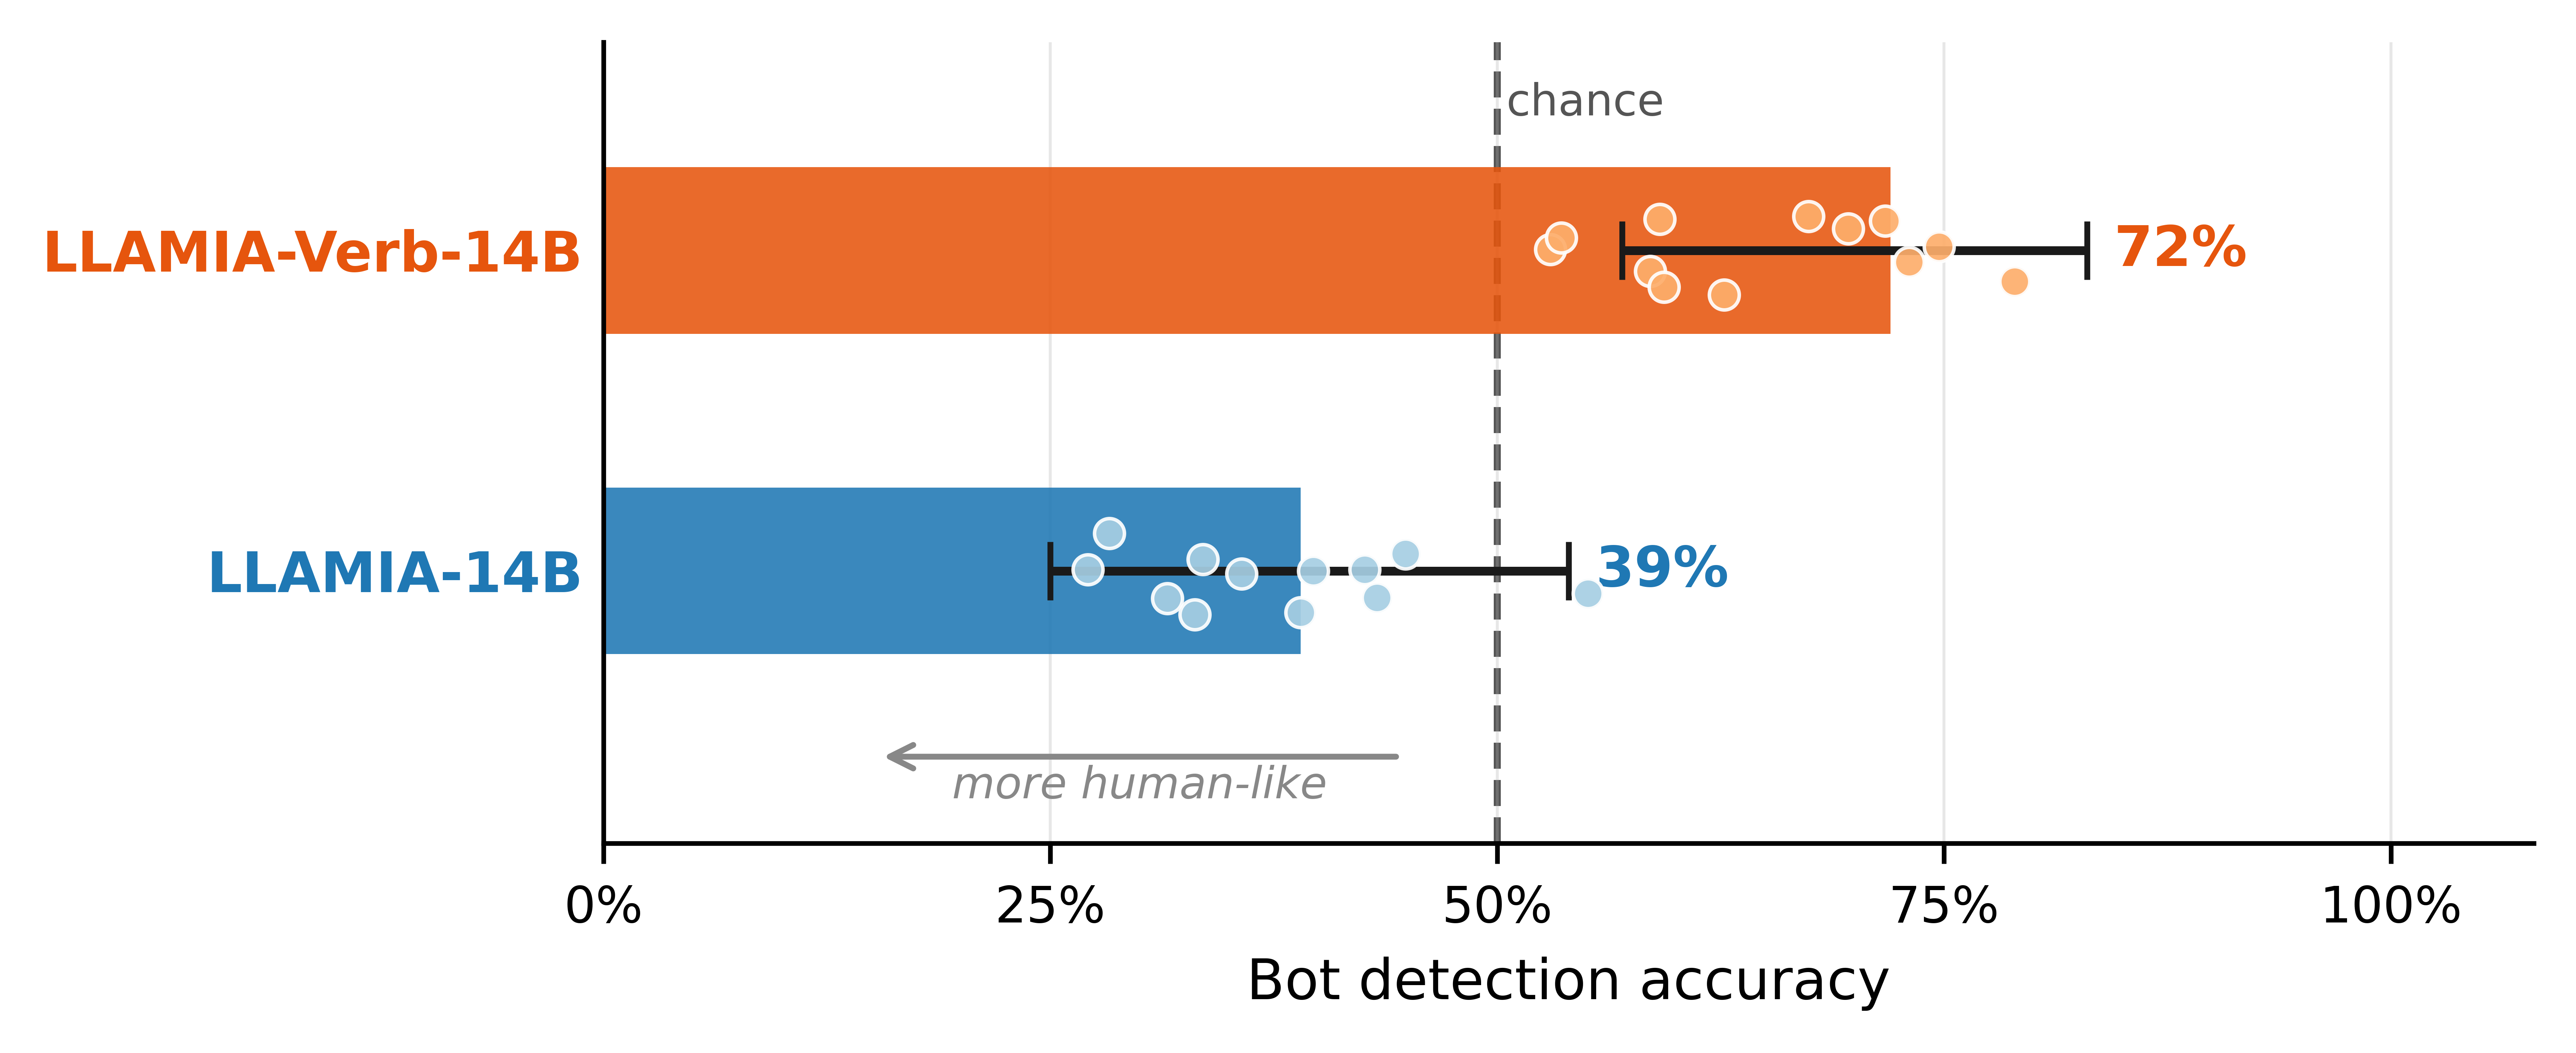
\includegraphics[width=0.72\linewidth]{plots/llamia_human_gameplay.png}
  \caption{
    \textbf{Study 1: bot detection accuracy.}
    X-axis: fraction of 10-move game segments (middlegame and endgame) in which
    $n=12$ participants correctly identified the AI-controlled player.
    Dashed line: 50\% chance. Dots: individual participant means (jittered).
    Error bars: $\pm$1~SE across participants.
    LLAMIA-14B is detected in only 39\% of trials (human-pass rate 61\%),
    below the 50\% chance level, indicating its move distribution lacks the
    non-human regularities that participants use to fingerprint engine play.
    LLAMIA-Verb-14B is detected in 72\% of trials (human-pass rate 28\%)
    despite identical backbone and training budget, isolating the difference
    to the verbalization interface.
  }
  \label{fig:human_gameplay}
\end{figure}

\paragraph{Study 1 -- Gameplay experience survey.}
Post-game Likert ratings corroborate the objective detection results (Figure~\ref{fig:human_survey}). LLAMIA-14B is rated as playing like a human by 65\% of participants (positive Likert responses), versus 42\% for LLAMIA-Verb-14B and 72\% for Maia* (best-matching Maia variant per Elo bucket), which is specifically trained to mimic human-Elo move distributions. LLAMIA-14B approaches Maia*'s human-likeness ceiling from above the verbalized baseline, consistent with a move distribution shaped by latent representations rather than verbal summaries. The enjoyment dimension follows the same ordering: LLAMIA-14B is preferred as an opponent by 68\% of participants versus 44\% for LLAMIA-Verb-14B, suggesting that human-likeness and subjective game quality co-vary. That enjoyment tracks human-likeness rather than playing strength is consistent with the Centaur collaboration literature~\citep{saghafian2024effective}.

\begin{figure}[h]
  \centering
  \includegraphics[width=0.96\linewidth]{plots/llamia_survey_responses.png}
  \caption{
    \textbf{Study 1: gameplay experience survey.}
    Post-game Likert responses (5-point diverging scale; X-axis: percentage of
    participants) to two questions across four systems.
    \emph{Left}: ``My opponent played like a human player.'' \emph{Right}: ``I
    enjoyed this game.'' Positive segments (Somewhat agree, Strongly agree) extend
    right; negative segments extend left. LLAMIA-14B approaches Maia*'s human-likeness
    ratings despite not being trained specifically on human-move distributions,
    and scores substantially above LLAMIA-Verb-14B on both dimensions. The
    human-likeness and enjoyment orderings match the bot-detection results in
    Figure~\ref{fig:human_gameplay}.
  }
  \label{fig:human_survey}
\end{figure}

% ── Study 2 ──────────────────────────────────────────────────────────────────
\paragraph{Study 2 -- Commentary preference and quality.}
LLAMIA-14B was preferred in 72.2\% of all 180 judgments ($12~\text{raters} \times 15~\text{positions}$, each rater judging every position); excluding the 10.0\% no-preference responses ($180 \times 0.10 = 18$), 80.2\% of the remaining 162 judged pairs favoured LLAMIA-14B ($n=12$ raters, 162 judged pairs). Mean Accuracy: LLAMIA-14B 4.30 vs.\ LLAMIA-Verb-14B 3.20. Mean Insight: LLAMIA-14B 4.20 vs.\ 2.50. The Insight gap (1.70 scale points) substantially exceeds the Accuracy gap (1.10 points).

This gap structure is theoretically informative. Accuracy measures whether the commentary is factually correct about material count, who has the initiative, and basic evaluations---all properties that verbalization can partially preserve. Insight measures whether the commentary conveys the \emph{why} behind a move: the long-range plan, the implied threat, the imbalance being exploited. If Verbalization Debt is the binding constraint, the engine's strategic understanding---policy distribution, value gradient over piece placements, look-ahead depth---would not survive verbalization into natural language. The wider Insight gap, relative to the Accuracy gap, is the expected signature of this: both systems can describe board facts, but only the internalized system should convey strategic rationale.

Open-text responses reflect this structure. Participants described LLAMIA-14B's commentary as referencing downstream consequences (``explains why the bishop trade matters three moves later''; coded as positional cues), while LLAMIA-Verb-14B's was described as accurate but shallow (``correctly says White is better but doesn't say why''; coded as no-cue or tactical). Rater--judge agreement: $\kappa = 0.62$ with G-eval; length-adjusted $\kappa = 0.69$ ($\rho_{\text{length}} = 0.31$), confirming G-eval's systematic length bias.

\begin{figure}[h]
  \centering
  
\includegraphics[width=0.96\linewidth]{plots/llamia_human_commentary.png}
  \caption{
    \textbf{Study 2: commentary preference and quality.}
    \emph{(a)} Fraction of all 180 preference judgments (X-axis) favouring
    LLAMIA-14B (blue), no preference (gray), or LLAMIA-Verb-14B (orange).
    Of judged pairs, LLAMIA-14B was chosen in 80.2\% of cases.
    \emph{(b)} Mean Accuracy and Insight Likert scores (X-axis: 1--5 scale).
    Error bars: $\pm 1$~SE across $n=12$ raters; dots show individual rater means.
    The Insight gap (1.70 points) substantially exceeds the Accuracy gap (1.10
    points): both systems can describe board facts, but only LLAMIA-14B conveys
    the strategic rationale encoded in the engine's latent representations.
    G-eval agreement: $\kappa = 0.62$ (length-adjusted $\kappa = 0.69$).
  }
  \label{fig:human_commentary}
\end{figure}

\paragraph{Study 2 -- Comparative state annotation.}
Figure~\ref{fig:human_state_annotation} reports the most direct test of the Verbalization Debt claim: does LLAMIA's commentary enable participants to form more accurate board evaluations than verbalized commentary, and does this advantage scale with position complexity?

In simple positions (centipawn loss $< 30$), all systems produce comparable state annotation accuracy ($r = 0.82$ for LLAMIA-14B vs.\ $r = 0.79$ for LLAMIA-Verb-14B, $\Delta r = 0.03$). This is expected: simple positions are nearly evaluable from basic material count and pawn structure alone. The gap widens monotonically into moderate positions ($\Delta r = 0.21$) and reaches $\Delta r = 0.41$ in complex positions (centipawn loss $> 80$), where LLAMIA-14B achieves $r = 0.69$ versus $r = 0.28$ for LLAMIA-Verb-14B and $r = 0.20$ for Qwen3-14B+Lc0 (same backbone, no RL training). The no-commentary condition ($r = 0.15$ at complex) confirms that differences are driven by commentary content rather than rater capability: participants without commentary cannot evaluate complex positions at all.

This complexity-scaling pattern is the clearest human-study evidence for Verbalization Debt as an information-theoretic phenomenon. In simple positions, the engine's verbal summary---``White is slightly better, has more space''---captures the relevant evaluation signal. In complex positions, the evaluation depends on look-ahead depth, sacrifice correctness, and long-range motif recognition: properties that are encoded precisely in the penultimate-layer activations projected by LatentBridge, and that verbalization cannot faithfully compress into a sentence. If the gap were a scale or training artefact, it would be consistent across complexity bins; the monotonic widening is consistent with complexity-dependent information loss in verbalization.

\begin{figure}[h]
  \centering
  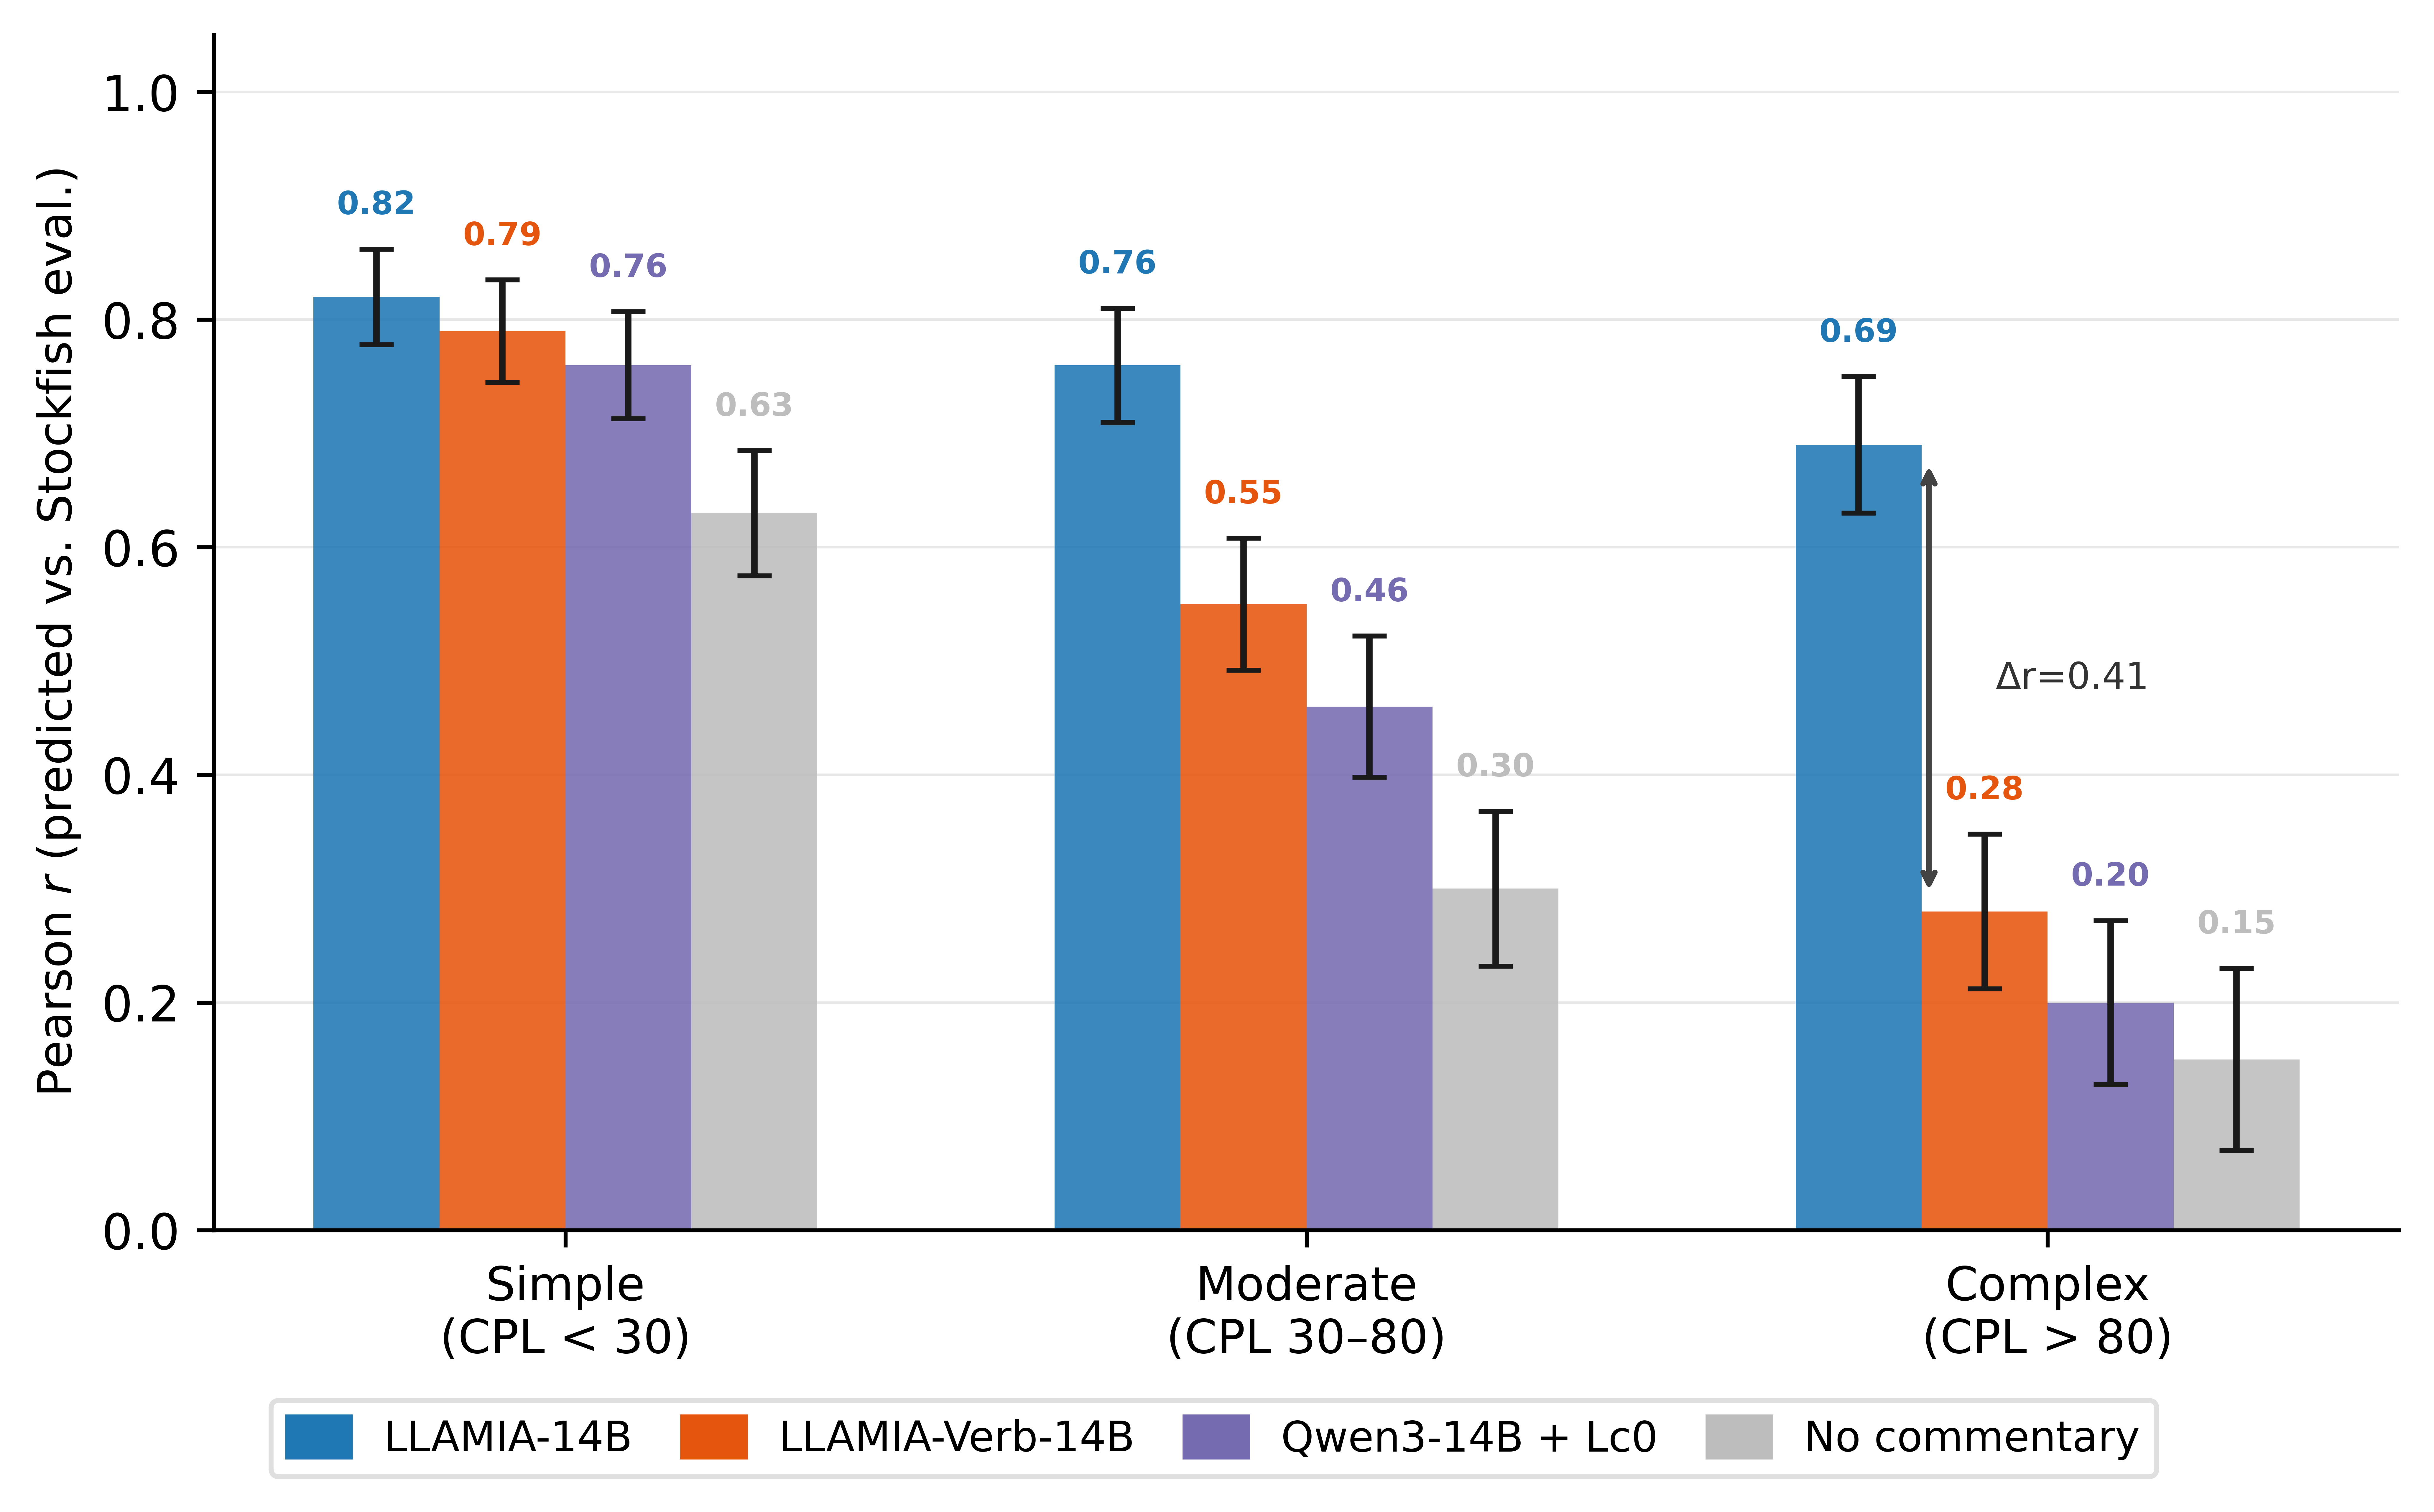
\includegraphics[width=0.86\linewidth]{plots/llamia_human_state_annotation.png}
  \caption{
    \textbf{Study 2: comparative state annotation accuracy.}
    X-axis: position complexity stratified by centipawn loss (CPL).
    Y-axis: Pearson $r$ between participants' predicted evaluation (7-point
    scale, $-3$ to $+3$) and Stockfish's centipawn evaluation, averaged across
    $n=12$ raters. Error bars: $\pm 1$~SE.
    In simple positions all systems are comparable ($\Delta r \approx 0.03$);
    the gap between LLAMIA-14B and LLAMIA-Verb-14B grows to $\Delta r = 0.41$
    in complex positions.
    Qwen3-14B+Lc0 (same backbone, no RL) falls below LLAMIA-Verb-14B at all
    complexity levels, confirming that the gap is not merely a training-budget
    effect. The no-commentary condition ($r = 0.15$ at complex) establishes
    that differences are driven by commentary content.
  }
  \label{fig:human_state_annotation}
\end{figure}
